\section{Baseline without Middleware (75 pts)}

In this section we study the performance characteristics of the memtier clients and memcached servers.

\subsection{One Server}

We aim to show how the behavior of one single server changes as we add more clients, with the setup listed below. Figure~\ref{fig:2.1_responsetime} is the response time measured by memtier with regard to the number of clients, for both read-only and write-only workloads. Figure~\ref{fig:2.1_throughput} is the corresponding throughput, along with the theoretical throughput from the number of clients and measured response time by the interactive law. By comparing it with the measured throughput, we can see that the interactive law holds in these experiments.

\begin{center}
	\scriptsize{
		\begin{tabular}{|l|c|}
			\hline Number of servers                & 1                        \\ 
			\hline Number of client machines        & 3                        \\ 
			\hline Instances of memtier per machine & 1                        \\ 
			\hline Threads per memtier instance     & 2                        \\
			\hline Virtual clients per thread       & \begin{tabular}{@{}c@{}}[1, 4, 8, 12, 16, 20, 24, 28, 32] \\ For write [36, 40, 44, 48] in addition \end{tabular} \\ 
			\hline Workload                         & Write-only and Read-only \\
			\hline Multi-Get behavior               & N/A                      \\
			\hline Multi-Get size                   & N/A                      \\
			\hline Number of middlewares            & N/A                      \\
			\hline Worker threads per middleware    & N/A                      \\
			\hline Repetitions                      & 3  $\times$ 80 seconds each          \\ 
			\hline 
		\end{tabular}
	} 
\end{center}

\begin{figure}[!h]
\parbox{.5\linewidth}{
\centering
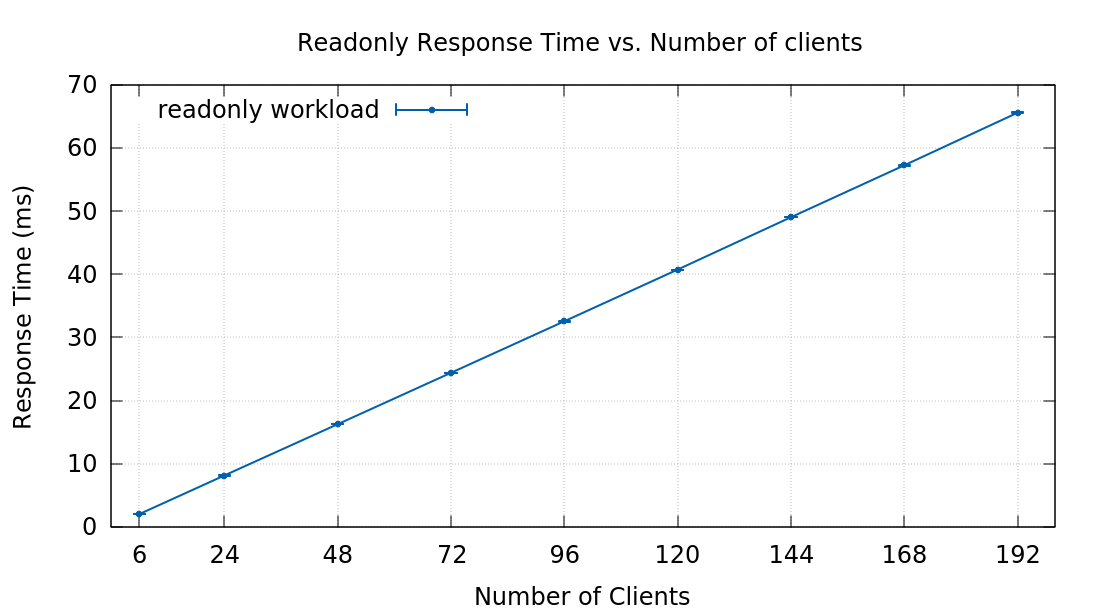
\includegraphics[width=0.5\textwidth]{img/2_1_responsetime_readonly.png}
}
\parbox{.5\linewidth}{
\centering
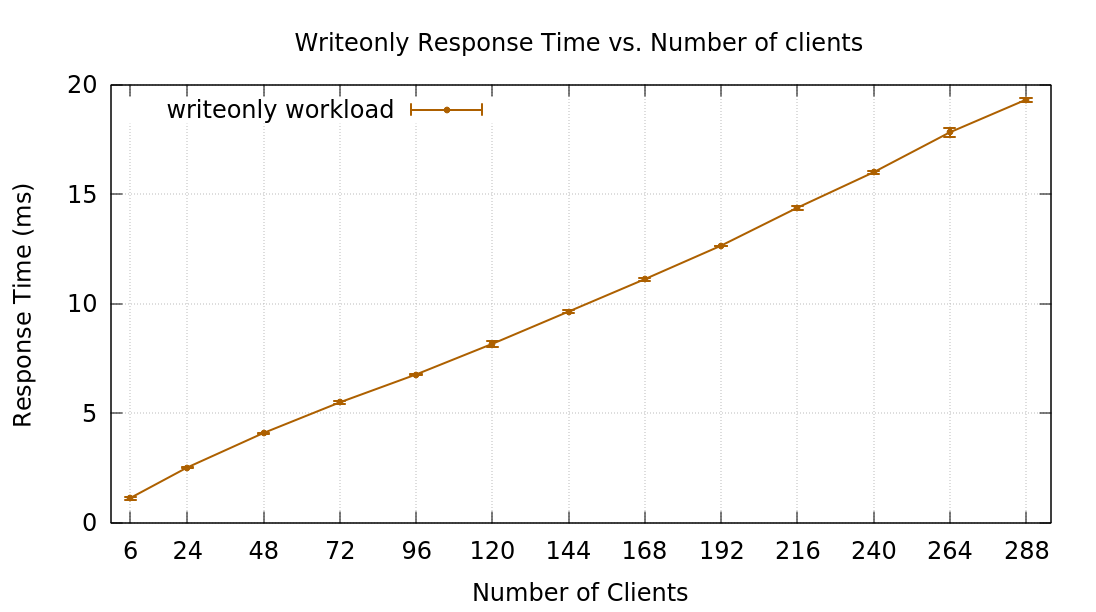
\includegraphics[width=0.5\textwidth]{img/2_1_responsetime_writeonly.png}
}
\captionsetup{justification=centering}
\caption{\label{fig:2.1_responsetime}Measured Response Time as a function of NumClients for One Server \\(Error bars are too small to be distinguished)}
% \end{figure}

% \begin{figure}[!h]
\parbox{.5\linewidth}{
\centering
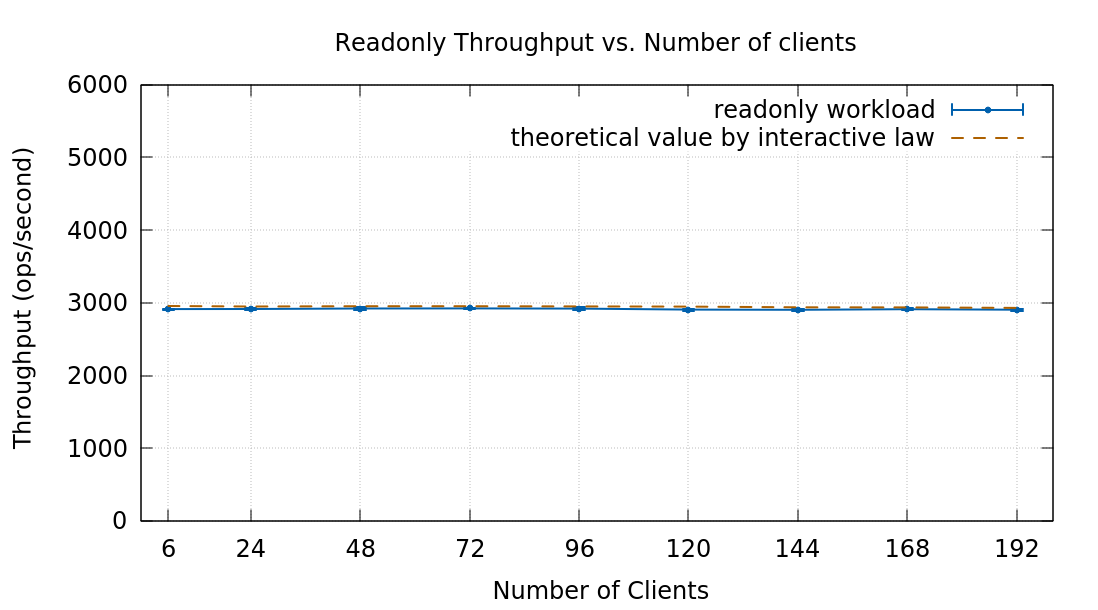
\includegraphics[width=0.5\textwidth]{img/2_1_throughput_readonly.png}
}
\parbox{.5\linewidth}{
\centering
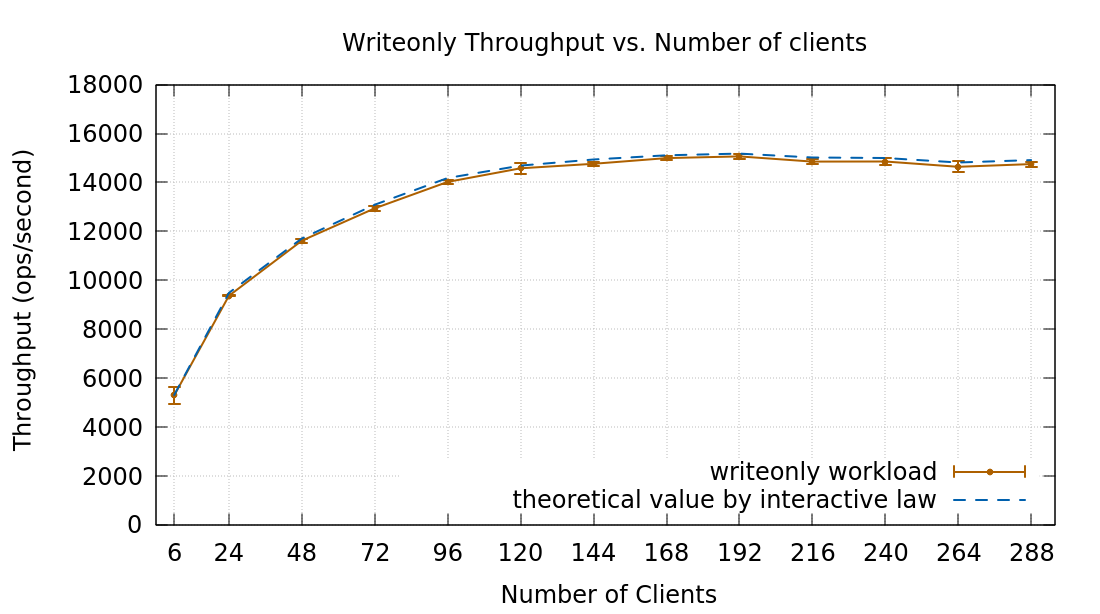
\includegraphics[width=0.5\textwidth]{img/2_1_throughput_writeonly.png}
}
\captionsetup{justification=centering}
\caption{\label{fig:2.1_throughput}Measured Throughput as a function of NumClients for One Server \\(Error bars are too small to be distinguished)}
\end{figure}

\subsubsection{Explanation}

For readonly workload, the system hits a maximum throughput of 2912.41 ops/second and becomes saturated even when there is only one virtual client in each memtier thread. No under-saturated phase is observed; all points after are over-saturating the system since the throughput does not change and the response time grows linearly with the number of clients. This is because the sending bandwidth of the server VM is limited at 100 Mbits/s, or 11.92 MiB/s, when the value size is 4096 Bytes (or full response size 4130 Bytes due to header and termination characters), this yields a maximum sending capacity of 3026.63 ops/second. We do not see 3000 on the plot because the results are actually average throughputs over the whole running period, which is not necessarily the maximum throughput at any second. However, we can still see from the server's \texttt{dstat} log that it indeed keeps sending a traffic of 12$\sim$13MB at each second, which proves that the bottleneck is really the server's uploading bandwidth.

For writeonly workload, when increasing clients from one per memtier thread (or 6 clients in total), the system gradually changes from under-saturation to saturation, and it becomes fully saturated at 120 clients with 14578.22 ops/sec, because there is barely no growth in throughput when adding more clients, while the response time grows linearly with the number of clients. The \texttt{dstat} log from server also supports this observation: when there are 120 clients, the CPU load becomes nearly 100\%, which means that the server has been fully utilized, and it has no more CPU power to spend.

Therefore, we conclude that for readonly workload, a server can support up to about 3000 ops/second, which is limited by its network sending bandwidth. For writeonly workload, a server can support up to about 15000 ops/second, which is limited by its CPU processing capacity.

\subsection{Two Servers}

Now we use two servers to test the capacity of a single load generating machine, with the experiment setup below. Figure~\ref{fig:2.2}, left is the response time measured by memtier with regard to the number of clients, for both read-only and write-only workloads. Figure~\ref{fig:2.2}, right is the corresponding throughput, along with the theoretical throughput from the number of clients and measured response time by the interactive law. By comparing it with the measured throughput, we can see that the interactive law also holds. 

% Use 1 load generating VM, with one memtier (CT=1) connected to each memcached instance (two memcache instances in total), and vary the number of virtual clients (VC) per memtier thread between 1 and 32. Show how the behavior of the server changes and explain what conclusions we can draw from this experiment.

\begin{center}
	\scriptsize{
		\begin{tabular}{|l|c|}
			\hline Number of servers                & 2                        \\ 
			\hline Number of client machines        & 1                        \\ 
			\hline Instances of memtier per machine & 2                        \\ 
			\hline Threads per memtier instance     & 1                        \\
			\hline Virtual clients per thread       & [1, 2, 3, 4, 5, 6, 8, 16, 32]                  \\ 
			\hline Workload                         & Write-only and Read-only \\
			\hline Multi-Get behavior               & N/A                      \\
			\hline Multi-Get size                   & N/A                      \\
			\hline Number of middlewares            & N/A                      \\
			\hline Worker threads per middleware    & N/A                      \\
			\hline Repetitions                      & 3 $\times$ 80 seconds each             \\ 
			\hline 
		\end{tabular}
	} 
\end{center}

\begin{figure}[!h]
\parbox{.5\linewidth}{
\centering
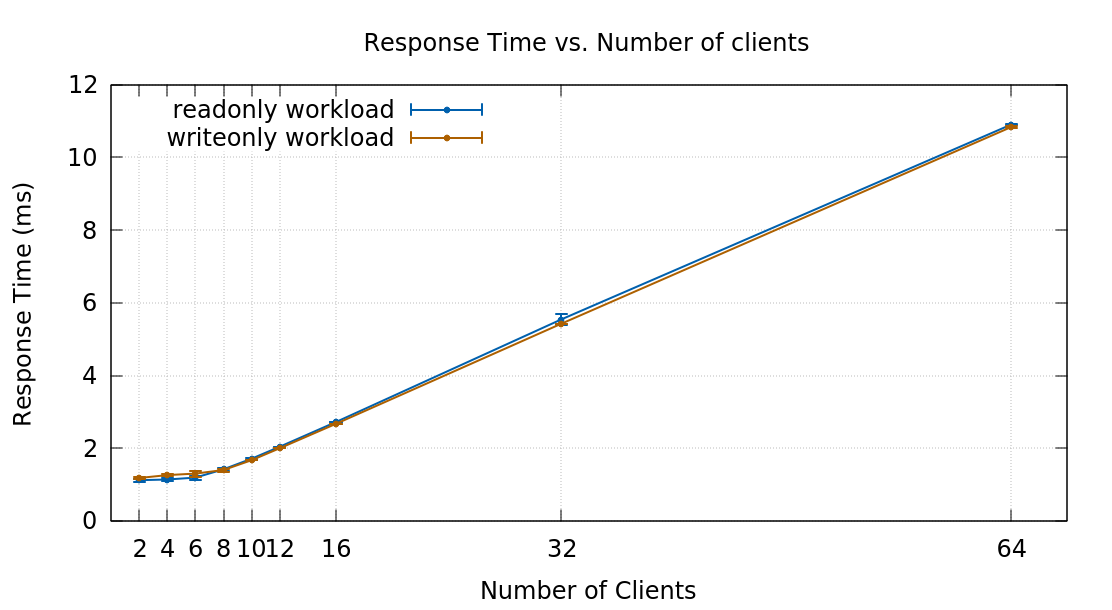
\includegraphics[width=0.5\textwidth]{img/2_2_responsetime.png}
}
\parbox{.5\linewidth}{
\centering
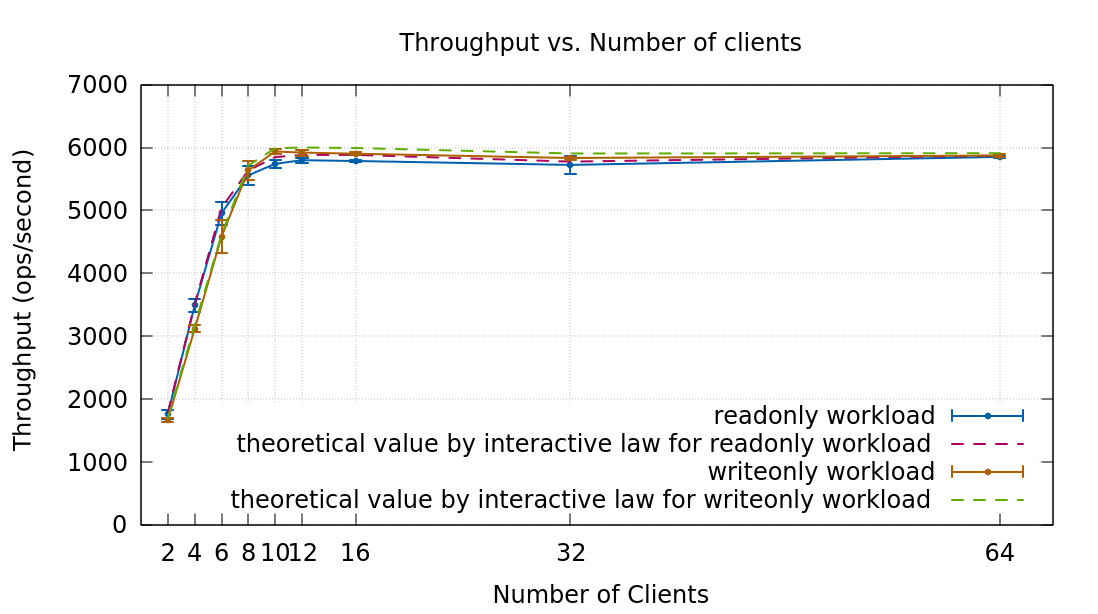
\includegraphics[width=0.5\textwidth]{img/2_2_throughput.png}
}
\captionsetup{justification=centering}
\caption{\label{fig:2.2}Measured Performance as a function of NumClients for Two Servers \\(Error bars are too small to be distinguished)}
\end{figure}

\subsubsection{Explanation}

The behaviours for readonly and writeonly workloads look very similar, as they both become saturated at 8 clients, reaching a throughput of about 5800 ops/second, and the response time grows linearly afterwards, without considerable growth in the throughput. However, the bottlenecks that cause saturation are really different.

For readonly workload, the maximum throughput is around two times the value in readonly experiments of the previous section, and the key reason is the same: the two servers send 4130 Bytes responses to clients, which makes its 100 Mbits/s sending bandwidth (or 200 Mbit/s in total) a bottleneck, limiting the maximum throughput at 6053 ops/second. The client machine is not a bottleneck, neither in CPU nor in network, which can be seen from its \texttt{dstat} logs.

However, for writeonly workload, it is the client that sends 4096 Bytes values to the servers (or 4128 Bytes requests). Since the sending bandwidth of a client machine is $\sim$200 Mbits/s, or 23.84 MiB/s, it limits the maximum writeonly throughput at 6056 ops/second. 

Again, the maximum throughput on the plot does not seem have a small gap with this value, this is because the plotted throughputs are averages over the 60 seconds experimenting period, which are not the maximum throughput at any second. Moreover, the throughput suffers from unstable network when the network bandwidth becomes fully utilized, possibly due to the management events of Azure VM hosts. This also lowers the average throughput over 60 seconds. But we can still prove network saturation from the servers' \texttt{dstat} logs that the sending speed is almost always 12$\sim$13 MiB/s on each server (for readonly) or 23$\sim$24 MiB/s on the client (for writeonly).

In conclusion, the readonly maximum throughput in this subsection is still limited by server bandwidth, thus it does not reveal the readonly capacity limit of the client machine. For writeonly workload, we successfully discovered the limit of the client machine, which has been bottlenecked by its sending bandwidth.

\subsection{Summary}

\begin{center}
	{Maximum throughput (ops/sec) of different VMs.}
	\begin{tabular}{|l|p{2cm}|p{2cm}|p{4cm}|}
		\hline                        & Read-only workload & Write-only workload & Configuration gives max. throughput \\ 
		\hline One memcached server   &   2912.41, $\sigma=7.83$     &  14578.22, $\sigma=234.82$        &                     VC = 6 for readonly, VC = 120 for writeonly         \\ 
		\hline One load generating VM &   5558.06, $\sigma=152.19$   &  5637.51, $\sigma=152.90$                &            VC = 8 for both                 \\ 
		\hline 
	\end{tabular}
\end{center}

%Write at least two paragraphs about how both results relate. Describe what is the bottleneck of this setup is. If the maximum throughput for both experiments is the same, explain why. If it is not the case, explain why not. Write down key take-away messages about the behaviour of the memtier clients and the memcached servers.

% How both results relate?
The one server experiments successfully show the limit of one memcached server under both read-only and write-only workloads, by using all three client machines to generate as much load as possible. On the other hand, the two servers (one client) experiments try to show the limit of one load generating machine, with the hope that as many as two servers will not be the bottleneck, but unfortunately the result shows this is not always true.

%Bottleneck?
In one server experiments, the bottleneck is always the server. For read-only workload, it is limited by a network sending bandwidth of 100 Mbits/s. For write-only workload, the network is no longer the bottleneck: it is limited by its CPU capacity.
In two servers experiments, the bottleneck is still the servers' sending bandwidth for read-only workload. For write-only workload, instead, it is limited by the client's sending bandwidth of 200 Mbits/s. Although the maximum throughput for both workloads is the same, the bottleneck under the hood is different.

% Why maximum throughput different?
The read-only maximum throughput for one client experiments is roughly two times that of one server (with standard deviation considered), because for read-only experiments the bottleneck is always the server, and we have doubled the number of servers in one client experiments.
The write-only maximum throughput for one client experiments is much lower than one server, because only one client machine is not enough to fully utilize the CPU of one server; the upload bandwidth of the client itself has become the bottleneck.

% Key take-away messages about the behaviour of the memtier clients and the memcached servers?

The key take-away messages about the behaviour of a memcached server is that its CPU capacity limits its write-only throughput to at most about 15000 ops/sec, and its sending bandwidth (11.92 MiB/s) limits its read-only throughput to at most about 3000 ops/sec. For a memtier client machine, its sending bandwidth (23.84 MiB/s) limits its write-only workload throughput to a maximum of about 6000 ops/sec; however, its limit on read-only workload is unknown because we did not use enough many servers to reach that.